\begin{figure}
\centering

\includegraphics[scale=.4]{Photos/FE1}
\end{figure}  
  
  
\textbf{INTELLIGENCE}\\
\textbf{Adieu Dr Dieu}


Vietnamese mathematician, long the most outspoken critic of the ruling Communist Party to remain out of prison, has been ousted from his post as vice-chairman of the National Centre for Scientific Research. In recent months, Dieu had called for the party to abandon its Marxist-Leninist ideology and challenged it to allow other parties to compete in the country’s political life. Officially, he was removed from his post in a dispute with the centre’s director physicist Nguyen Van Hieu, but observers see Dieu’s firing as an attempt by the party to isolate him from potential supporters, Dieu has asked to be allowed to teach mathematics and computer science at Hanoi University. 




\textbf{VIETNAM}\\

 Mon Dieu!


\textbf{FROM OUT SOUTH-EAST ASIA CORRESPONDENT    \quad           HANOI}


Sitting in his book-lined study in Hanoi, Phan Dinh Dieu looks the very model of academic detachment. Mr Dieu is a professor of mathematics and a respected figure in Hanoi. But he is also probably the most outspoken advocate of political reform in Vietnam to remain out of prison. 


In recent years the number of political prisoners has decreased. All the same, Asia Watch, an American human-rights group, estimates that Vietnam has “hundreds if not thousands of political and religious prisoners”. This year eight dissidents were jailed for circulating a newsletter called \textit{Freedom Forum}, which called  for multi-party democracy. Doan Viet Hoat, the group’s leading figure, got 15 years. 


As a man who spent the Vietnam war in the north and who has worked within the system (without ever joining the Communist Party), Mr Dieu is granted some latitude. But he recently lost his job as vice-president of the National Centre for Scientific Research in Hanoi. The official reason is that he had a dispute with the centre’s director, but some think that the party may be trying to isolate Mr Dieu from students. Still, somebody in the government is clearly not averse to giving Mr Dieu a platform. His meeting with \textit{The Economist} was arranged by the foreign ministry’s press service and watched over by an official guide. 


Alongside the learned papers and football magazines on Mr Dieu’s shelves are the works of Vaclav Havel and Andrei Sakharov. This is an act of boldness in itself. The evidence used against convicted dissidents has included articles in their possession about the upheavals in Eastern Europe. For Vietnam’s leader the lesson of Eastern Europe was clear: press ahead with economic reform but keep politics frozen. Mr Dieu is inclined to disagree, although he is careful to offer his views as part of a scientific rather that a political debate. He says, 
\begin{quote}
\textit{The threat of chaos is real in Vietnam, and the concern of people in the party is to achieve stability. I agree that we need stability, but of what kind? Scientifically, we can differ on that, they have a static view a stability. A more scientific concept is dynamic stability achieved through evolution. It is impossible in principle to have economic development and not have political development. The market economy contradicts communism. If you accept market economics sooner or later you have to abandon the principles of communist society: one unique party in power, the dominant role of the public sector and so on. }
\end{quote}

Some theorists in Asia suggest that communism in Vietnam and China will not collapse as it has in Eastern Europe. They believe economic reform can be combined with single-party rule for years to come. The ruling parties will simply ditch the ideological baggage of communism and adopt the authoritartianism of Singapore or Taiwan. 


Mr Dieu is not convinced. Like most patriotic Vietnamese, he instinctively shies away from any comparison to China. Nor are Singapore and Taiwan good models, according to Mr Dieu. “The ruling parties there evolved in very different circumstances from today. The spirit of democracy is now much stronger in our area than it was 20 years ago.” Events in Taiwan this week (see page 25) tend to support his view. 


Mr Dieu is hopeful about the growth of pluralism in Vietnam. He says that discussions within the party are much freer than they were a couple of years ago; it is now possible to study the principles of social democracy or the crisis of Marxism. At official seminars concepts like multi-party democracy have been aired. “We can discuss these things in private. Whether the party accepts them or not is another matter,” he says, amid gales of nervous laughter. 

\begin{figure}
\centering
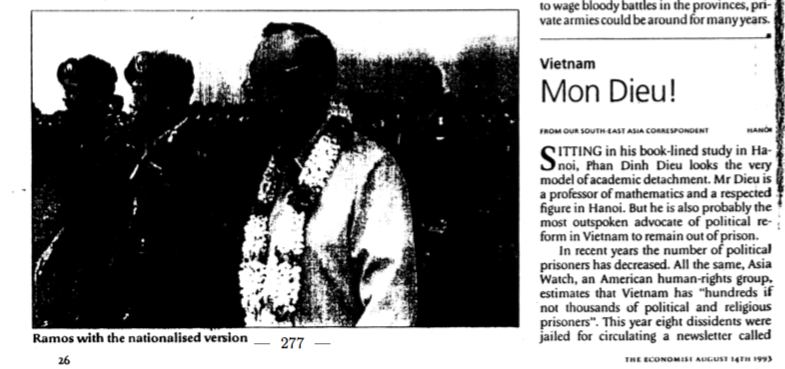
\includegraphics[scale=.4]{Photos/FE2}
\end{figure}  
  

\newpage
TIN TÌNH BÁO


Tạm biệt Giáo sư Diệu (Adieu Dr Dieu)


Nhà toán học Việt Nam, nhà phê bình kiên trì và thẳng thắn nhất về Đảng Cộng sản đang cầm quyền chưa khi nào bị tù đày nhưng đã bị giáng chức Phó Viện Trưởng Viện Hàn Lâm Khoa Học Việt Nam. Những tháng gần đây, giáo sư Diệu đã kêu gọi Đảng cộng sản hãy từ bỏ ý thức hệ Marxist-Leninist và để cho các đảng khác có cơ hội canh tranh trong đời sống chính trị của đất nước. Lý do chính thức khiến ông đã bị giáng chức sau khi tranh luận với vị Giám đốc Trung tâm cũng là nhà vật lý tên là Nguyễn Văn Hiệu. Tuy nhiên các nhà quan sát nhận định việc cho ông Diệu thôi chức tước là để cô lập ông với các nhà ủng hộ tiềm năng. Giáo sư Diệu cũng yêu cầu được tiếp tục công việc giảng dạy toán học và khoa học máy tính tại trường Đại học ở Hà nội. 


\noindent \textbf{VIỆT NAM}\\
Ông Diệu


\begin{center}
PHÓNG VIÊN TỪ TRUNG TÂM ĐÔNG NAM Á - HÀ NỘI 
\end{center}

Ngồi cùng ông trong căn phòng đầy sách tại Hà Nội, Giáo sư Phan Đình Diệu toát lên dáng vẻ của một nhà học thuật độc lập. Ông là một Giáo sư toán học và là một gương mặt đáng kính ở thủ đô Hà Nội. Nhưng ông cũng là người ủng hộ thẳng thắn nhất cho cải cách chính trị ở Việt Nam mà vẫn được tự do. 


Trong những năm gần đây số lượng tù nhân chính trị đã giảm. Cùng nhận xét trên, Asia Watch - tổ chức nhân quyền của Mỹ ước tính Việt Nam có "hàng trăm nếu không muốn nói là hàng ngàn tù nhân chính trị và tôn giáo". Năm nay, tám nhà bất đồng chính kiến bị bắt giam vì đã phát hành trang tin có tên Diễn đàn Tự Do kêu gọi dân chủ đa nguyên đa đảng dưới sự khởi xướng của ong Đoàn Viết Hoạt - người đã phải nhận mức án 15 năm tù. 


Là người đã từng tham gia chiến đấu ở miền Bắc Việt Nam và làm việc trong hệ thống (chưa bao giờ gia nhập Đảng Cộng sản), Giáo sư Diệu cũng được trao một số quyền nhất định, tuy nhiên gần đây ông đã bị mất chức Phó Viện Trưởng Viện Hàn Lâm Khoa Học Việt Nam. Lý do chính thức đưa ra là ông đã có một cuộc tranh cãi với vị Giám đốc Trung tâm này tuy nhiên nhiều người cho rằng có lẽ Đảng muốn tách giáo sư Diệu khỏi sinh viên. Rõ ràng nhiều vị trong chính phủ tỏ rõ thái độ không muốn dành cho ông Diệu bất kỳ diễn đàn nào. Cuộc gặp của ông với tờ báo Kinh tế gia là do cơ quan báo chí thuộc Bộ ngoại giao sắp đặt và luôn bị giám sát. 


Cùng với các bài báo đã đọc và một số tạp chí bóng đá trên giá sách tại nhà giáo sư còn có các tác phẩm của Vaclav Havel và Andrei Sakharov. Đây có thể nói là một hành động táo bạo. Bằng chứng để chống lại các nhà bất đồng chính kiến đã ​​bị kết án gồm các bài viết của chính họ về cuộc binh biến ở Đông Âu. Và các nhà lãnh đạo của Việt Nam đã có một bài học rõ ràng từ Đông Âu là thúc ép đổi mới kinh tế nhưng chính trị thì bất động. Ông tỏ rõ thái độ bất đồng quan điểm trên mặc dù ông rất thận trọng khi đưa ra quan điểm của mình với góc nhìn của một nhà khoa học hơn là một cuộc tranh luận chính trị.


Mối đe dọa về sự bất ổn ở Việt Nam là có thật và mối quan ngại của nhiều người trong Đảng cộng sản là làm sao phải giữ được sự ổn định. Tôi hoàn toàn nhất trí việc chúng ta phải có sự ổn định nhưng ổn định như thế nào?. Về mặt khoa học, chúng ta cần phân biệt rõ là họ có một cái nhìn cố định về sự ổn định. Một khái niệm khoa học là cần phải đạt được sự ổn định trong thể động thông qua tiến trình vận động. Về mặt nguyên lý, không thể có một sự phát triển kinh tế tách rời sự vận động của chính trị. Kinh tế thị trường mâu thuẫn với chủ nghĩa cộng sản. Nếu anh chấp nhận nền kinh tế thị trường thì sớm hay muộn anh cũng phải dừng ngay các nguyên lý của xã hội cộng sản đó là tồn tại duy nhất một Đảng, vai trò phủ bóng của khu vực công và nhiều điều khác. 


Một số nhà lý thuyết ở châu Á cho rằng chủ nghĩa cộng sản ở Việt Nam và Trung Quốc sẽ không sụp đổ như ở Đông Âu. Họ cho rằng cải cách kinh tế có thể được kết hợp với sự nắm quyền hành của một đảng trong nhiều năm tới. Một cách đơn giản là các đảng cầm quyền chỉ cần dẹp đi mớ lý luận về chủ nghĩa cộng sản và thích nghi ngay với chủ nghĩa độc đoán như của Singapore hoặc Đài Loan.


Việc lý giải như vậy không thuyết phục được Giáo sư. Giống như hầu hết người Việt Nam yêu nước, ông tránh xa mọi so sánh với Trung Quốc, Singapore hay Đài Loan vì theo Ông: “Các đảng cầm quyền đang vận động theo bối cảnh khác nhau không giống với ngày nay. Hiện nay tinh thần dân chủ đang dần lớn mạnh trong khu vực so với 20 năm trước”. Các sự kiện trong tuần qua tại Đài Loan (xem trang 25) minh họa cho quan điểm của Giáo sư.


Giáo sư luôn hy vọng về sự phát triển đa nguyên, đa đảng ở Việt Nam. Ông nhận định các cuộc thảo luận trong nội bộ Đảng giờ đây đã cởi mở hơn so với cách đây nhiều năm. Giờ là lúc có thể nghiên cứu về các nguyên lý của dân chủ xã hội hoặc cuộc khủng hoảng của chủ nghĩa Mác. Tại các cuộc họp quan chức cũng đã xuất hiện những tiếng nói về nền dân chủ đa đảng. Giáo sư vừa nói vừa cười sảng khoái: “Chúng ta có thể thảo luận những vấn đề trên theo một cách riêng. Còn việc Đảng có chấp nhận hay không là một việc khác”./. 
